% Created 2024-01-20 Sat 13:16
% Intended LaTeX compiler: xelatex
\documentclass[11pt]{article}
\usepackage{graphicx}
\usepackage{longtable}
\usepackage{wrapfig}
\usepackage{rotating}
\usepackage[normalem]{ulem}
\usepackage{amsmath}
\usepackage{amssymb}
\usepackage{capt-of}
\usepackage{hyperref}
\usepackage{minted}
\usepackage[margin=2cm]{geometry}
\input{~/.doom.d/fancyLatexTemplate.tex}
\author{Spyridon Baltsas - AEM: 10443}
\date{}
\title{Parallel and Distributed Systems - CUDA Ising Model Report}
\hypersetup{
 pdfauthor={Spyridon Baltsas - AEM: 10443},
 pdftitle={Parallel and Distributed Systems - CUDA Ising Model Report},
 pdfkeywords={},
 pdfsubject={},
 pdfcreator={Emacs 28.2 (Org mode 9.6.1)}, 
 pdflang={English}}
\usepackage[style=ieee]{biblatex}
\addbibresource{/media/spyros/Data/sbalt/vs/Parallel and Distributed Systems/Ising Model CUDA/report/bibliography.bib}
\begin{document}

\maketitle

\section{Summary}
\label{sec:orge8ba27a}
This report is about my proposed solutions for impelementing the Ising Model in both CPU and GPU. To be more specific, here are briefly presented and explained the algorithms I have implemented for my approach, for both single CPU process and GPU parallelization use cases. Moreover, we will examine the overall performance, efficiency and scalability of all algorithms using the required charts and tables. The source code, building instructions and the usage of the produced binaries are available in \href{https://github.com/thetonk/pds-solutions/tree/main/Ising\%20Model\%20CUDA}{\emph{this repository}} and its \href{https://github.com/thetonk/pds-solutions/blob/main/Ising\%20Model\%20CUDA/README.md}{\emph{README}}.

\section{The model}
\label{sec:org714d894}
\subsection{Introduction}
\label{sec:org461d0e1}
The Ising Model is a statistical mechanics model for ferromagnetic materials. The model consists of discrete variables having only two possible values (-1,+1), representing the magnetic dipoles within the material. After finite time, it reaches an equilibrium with regions of positive and negative magnetic moments (spin). \autocite{enwiki:1191997935}
\subsection{Simulation}
\label{sec:orgc9bc6b7}
Thanks to its discrete nature, we may simulate the mentioned model using a cellular automaton. This cellular automaton for its operation is using von-Neumann (cross) neighbouring \autocite{enwiki:1196338105}, periodic, cyclic, boundary conditions and the following rule applied for each cell, let k be the iterations;
\begin{equation}
\label{eq:2}
M_{k+1}[i][j] = sign(M_{k}[i,j] + M_{k}[i-1][j] + M_{k}[i+1][j] + M_{k}[i][j-1] + M_{k}[i][j+1])
\end{equation}
\section{Approach}
\label{sec:orgf701648}
Please note that for all the following algorithms, the lattice matrix is represented using row-major order \autocite{enwiki:1161536790}. That is, if we have a \(n \times n\) matrix, the element \(a_{ij}\) can be accessed using the following formula, avoiding the complexity of using double pointers.
\begin{equation}
\label{eq:1}
a_{ij} =  M_{n \times n}[i][j] = M_{n \times n}[n \cdot i + j]
\end{equation}
Last but not least, in order to reduce memory usage as much as possible, all lattice matrices contain 1 byte only integers.
\subsection{Sequential}
\label{sec:orgc995e3a}
The sequential implementation is quite straightforward. First of all, two arrays are created, one for the current lattice state, and one for the next lattice state. Next, every element of next state lattice is calculated using the rule (\ref{eq:2}). Also a helper \texttt{temp} pointer is used to swap those two arrays on every iteration, in order the next state to be the current one and continue the calculations. The time complexity of this algorithm is \(\mathcal{O}(n^{2})\).
\subsection{CUDA parallelism}
\label{sec:org95ea536}
\subsubsection{V1}
\label{sec:orgb83034f}
For this version, we load array to the GPU global memory,and gets splitted into one-dimensional blocks. Each block contains a number of threads, and each thread is responsible for calculating the next lattice value of their corresponding element (one-to-one thread - element relationship). Therefore, there is no need for a double loop for this calculation anymore. Row, column and ID of the element can be found from the following snippet;
\begin{minted}[breaklines=true,breakanywhere=true,linenos=true,fontsize=\scriptsize]{cuda}
size_t elementID = blockDim.x*blockIdx.x + threadIdx.x;
size_t row = elementID / n, column = elementID % n;
\end{minted}
Afterwards, the logic is similar to sequential, but without the double loop, by directly reading from the GPU global memory.
\subsubsection{V2}
\label{sec:org55afa9a}
For this version, in order to prepare for the final version version, lattice matrix is splitted using smaller squares. As a result, this time, two-dimensional blocks are required, with 1 thread each. Also, for V2 and V3 block size is the number of rows of the sub-square.
\begin{center}
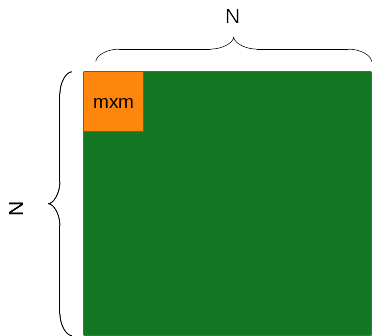
\includegraphics[height=120]{./images/cuda-square-split.png}
\captionof{figure}{\label{fig:1}Splitting lattice matrix in smaller sub-squares}
\end{center}
As a result, this time we need again a double loop to calculate each element of the sub-square. However, depending of the size of lattice matrix, may not fit perfectly in subsquares. The starting position of the loops and the required iteration which are depended on the size of lattice are calculated using the following snippet;
\begin{minted}[breaklines=true,breakanywhere=true,linenos=true,fontsize=\scriptsize]{cuda}
size_t blockRow = blockIdx.y*blockSize*n;
size_t blockCol = blockIdx.x*blockSize;
size_t rowIterations = n - blockRow/n < blockSize ? n-blockRow/n : blockSize;
size_t colIterations = n - blockCol < blockSize ? n- blockCol : blockSize;
\end{minted}
Again, like on V2, for the calculations we read directly from global memory. However, this algorithm isn't as efficient, since we use only 1 thread per square and not taking the most of GPU, but still much faster than sequential.
\subsubsection{V3}
\label{sec:orgde8bd2a}
For this version, we use again squares like on V2 as shown on figure \ref{fig:1}. This time, though, each element of the sub-square is assigned to a single thread, and calculations use the shared memory instead of the global. Thus, for this implementation we need again 2D blocks but with threads on both dimensions. With this implementation, like V1, there is no need for double loops, only checks whether we are within the limits of the lattice or not. The position of each element in the lattice matrix can be found by the following snippet;
\begin{minted}[breaklines=true,breakanywhere=true,linenos=true,fontsize=\scriptsize]{cuda}
size_t blockRow = blockIdx.y*blockDim.y;
size_t blockCol = blockIdx.x*blockDim.x;
size_t localRow = threadIdx.y, localCol = threadIdx.x, globalRow, globalCol;
globalCol = blockCol + localCol;
globalRow = blockRow + localRow;
\end{minted}
\begin{enumerate}
\item Shared memory storage design
\label{sec:orgd7929df}

In the shared memory 2D array, we must include all the elements of the sub-square, plus the neighboring elements of the sub-square. Also, for ease of calculations later, the elements of the subsquare must be in the middle, resulting in the following storage design. The elements in orange are the elements of the subsquare, and the elements in blue are the neighbors. In order to contain the neighbours of a \(m \times m\) square, a \((m+2) \times (m+2)\) square is needed.
\begin{center}
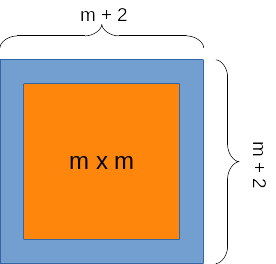
\includegraphics[height=120]{./images/cuda-subsquare.png}
\captionof{figure}{\label{fig:2}Shared memory array.}
\end{center}
\end{enumerate}
\section{Test specifications}
\label{sec:orgaacf3d7}
Please note that for the production of the following times, initial random state generation and I/O operations like loading data to RAM or GPU memory is ommited. For the GPU runs, \href{https://hpc.it.auth.gr/}{Aristotelis-HPC} (Aristotle University High-Performance Computing infrastructure) was used. To be exact, the CUDA was run to a NVIDIA Tesla P100 (12 GB VRAM) \autocite{hpc-resources}. For the sequential runs, an Intel Core i5-8300H @ 2.30 GHz (4 cores, 8 threads) was used.
\section{Results}
\label{sec:org8d4d9ee}
In the following results, N are the rows of square lattice and k the iterations. In addition, V2 and V3 were tested for block size equal to 16. In order to get maximum performance for each N, block size must be fine tuned by picking a value from 1 to 32, since 1024 threads are available for each block. For more detailed times of CUDA, please check the tables section.
\pagebreak
\subsection{Charts}
\label{sec:orgc9a3eb2}
\subsubsection{N variable, k constant}
\label{sec:org92640e7}
\begin{center}
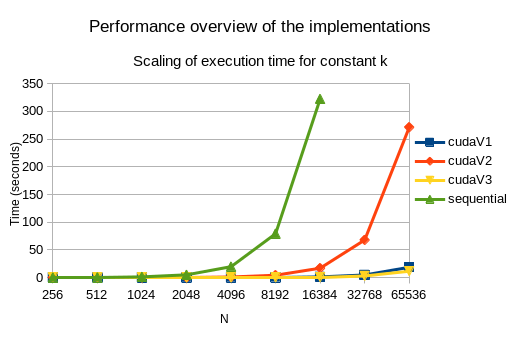
\includegraphics[height=200]{./images/performance-overview.png}
\captionof{figure}{Performance of sequential and CUDA implementations for k = 50}
\end{center}
\subsubsection{k variable, N constant}
\label{sec:orga21fd82}
\begin{enumerate}
\item Sequential
\label{sec:org55f4fe8}
\begin{center}
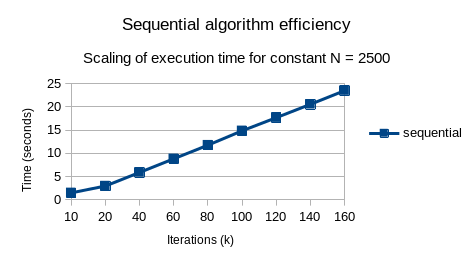
\includegraphics[height=200]{./images/seq-efficiency.png}
\captionof{figure}{Scaling efficiency for sequential algorithm, N = 2500}
\end{center}
\pagebreak
\item CUDA
\label{sec:org1b1f111}
\begin{center}
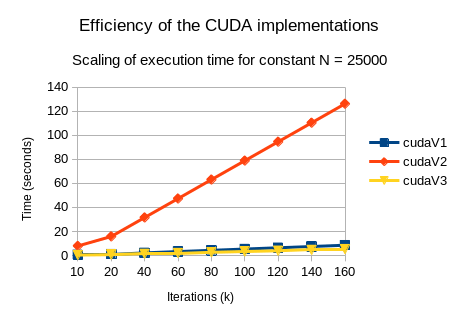
\includegraphics[height=200]{./images/cuda-efficiency.png}
\captionof{figure}{Scaling efficiency of CUDA algorithms, N = 2500}
\end{center}
\end{enumerate}
\subsubsection{V2 optimal block size}
\label{sec:org70c7b46}
\begin{center}
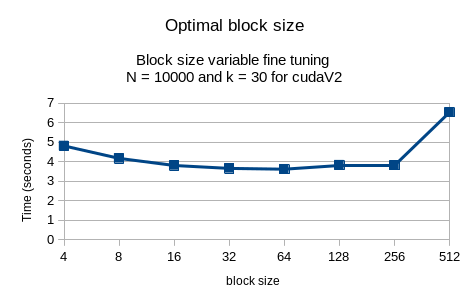
\includegraphics[height=200]{./images/block-size-effect.png}
\captionof{figure}{Optimizing block size}
\end{center}
\pagebreak
\subsection{CUDA Tables}
\label{sec:org6a7c35e}
\begin{table}[htbp]
\caption{Performance of CUDA algorithms for increasing N and k = 50, in seconds. Speedup compared to sequential}
\centering
\begin{tabular}{rrrrrrrr}
\hline
N & cudaV1 & cudaV2 & cudaV3 & sequential & speedup V1 & speedup V2 & speedup V3\\[0pt]
\hline
256 & 0.000792 & 0.012446 & 0.000418 & 0.108759 & 137 & 9 & 260\\[0pt]
512 & 0.001701 & 0.021732 & 0.001039 & 0.313754 & 184 & 14 & 302\\[0pt]
1024 & 0.005301 & 0.081199 & 0.00348 & 1.239513 & 234 & 15 & 356\\[0pt]
2048 & 0.019266 & 0.291012 & 0.01173 & 4.932072 & 256 & 17 & 420\\[0pt]
4096 & 0.074887 & 1.067174 & 0.0454 & 19.716256 & 263 & 18 & 434\\[0pt]
8192 & 0.294068 & 4.245557 & 0.179794 & 79.216957 & 269 & 19 & 441\\[0pt]
16384 & 1.166208 & 16.963191 & 0.717332 & 322.408843 & 276 & 19 & 449\\[0pt]
32768 & 4.649675 & 67.834809 & 2.878595 &  &  &  & \\[0pt]
65536 & 18.582241 & 271.312043 & 11.475189 &  &  &  & \\[0pt]
\hline
\end{tabular}
\end{table}

\begin{table}[htbp]
\caption{Scaling efficiency of CUDA algorithms for increasing k and N = 2500, in seconds. Speedup compared to sequential}
\centering
\begin{tabular}{rrrrrrrr}
\hline
k & cudaV1 & cudaV2 & cudaV3 & sequential & speedup V1 & speedup V2 & speedup V3\\[0pt]
\hline
10 & 0.006229 & 0.090122 & 0.004076 & 1.476218 & 237 & 16 & 362\\[0pt]
20 & 0.011678 & 0.177274 & 0.007373 & 2.948892 & 253 & 17 & 400\\[0pt]
40 & 0.022607 & 0.333522 & 0.013954 & 5.884672 & 260 & 18 & 422\\[0pt]
60 & 0.033550 & 0.507095 & 0.020553 & 8.820939 & 263 & 17 & 429\\[0pt]
80 & 0.044474 & 0.655744 & 0.027141 & 11.75787 & 264 & 18 & 433\\[0pt]
100 & 0.055405 & 0.818406 & 0.033747 & 14.861252 & 268 & 18 & 440\\[0pt]
120 & 0.065018 & 0.962793 & 0.040337 & 17.692676 & 272 & 18 & 439\\[0pt]
140 & 0.077054 & 1.123058 & 0.046943 & 20.574601 & 267 & 18 & 438\\[0pt]
160 & 0.087815 & 1.285326 & 0.053522 & 23.527411 & 268 & 18 & 440\\[0pt]
\hline
\end{tabular}
\end{table}

\printbibliography[heading=bibnumbered]
\end{document}